\newpage

\begin{center}
    \uppercase{Hoofdgerecht}
\end{center}
\rule{\linewidth}{0.4pt}
\subsection{Couscous familierecept}
\rule{\linewidth}{0.4pt}

\hspace{0.5cm}

\begin{paracol}{2}

\uppercase{\textbf{Ingrediënten}}

\hspace{0.25cm}

4-6 personen

\hspace{0.5cm}

\begin{itemize}
    \setlength\itemsep{0em}
    \item 2 uien
    \item 3 tenen knoflook
    \item Handje rozijnen
    \item 2-3 eieren
    \item 2 groentebouillonblokjes
    \item 1 winterpeen
    \item 1 knolselderij
    \item 1 courgette
    \item 1 (fles)pompoen
    \item Rozijnen
    \item Kikkererwten
    \item Tuinbonen
    \item Couscous
    \item +/- 1 kg kippenbouten of drumsticks
    \item 2 el olijfolie
    \item 2 tl kurkuma
    \item 2 tl gemalen koriander
    \item 1 tl komijnpoeder
    \item 1 tl karwijzaadpoeder
    \item 1 tl paprikapoeder
    \item \textonehalf tl gemberpoeder
    \item \textonehalf tl zwarte peper
\end{itemize}

\hspace{1cm}\newline
\uppercase{\textbf{Notities}}
\hspace{1cm}\newline
\begin{itemize}
    \setlength\itemsep{1em}
    \item In plaats van kip kan ook vlees gebruikt worden of niets (vega). \textbf{Het marineren hiervan kan de dag van tevoren al, maar het liefst een paar uur voor het maken van de couscous.}
    \item Met de groenten kan gevarieerd worden. Paprika is ook erg lekker, maar ook bosui erdoor.
\end{itemize}

\newpage % remove this when the images should start directly below 'Notities'

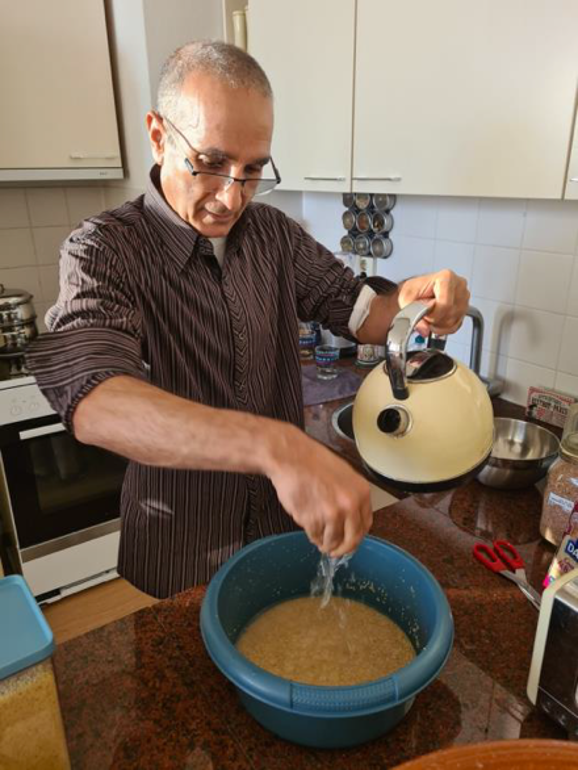
\includegraphics[width=\linewidth]{hoofdgerechten/fotos/couscous2.png}
\hspace{1cm}\newline
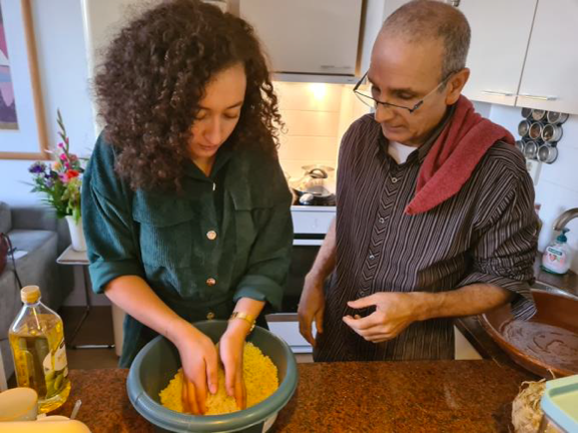
\includegraphics[width=\linewidth]{hoofdgerechten/fotos/couscous3.png}
\hspace{1cm}\newline
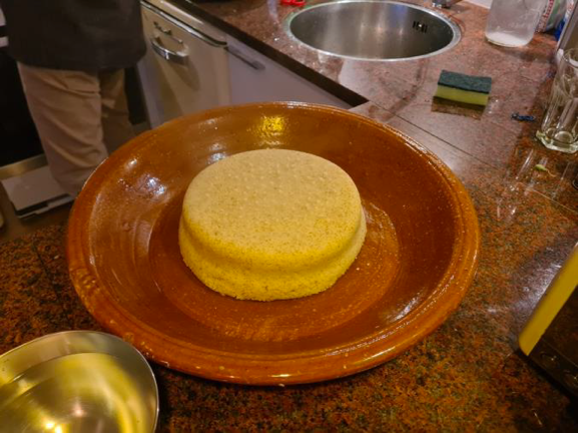
\includegraphics[width=\linewidth]{hoofdgerechten/fotos/couscous4.png}
\hspace{1cm}\newline
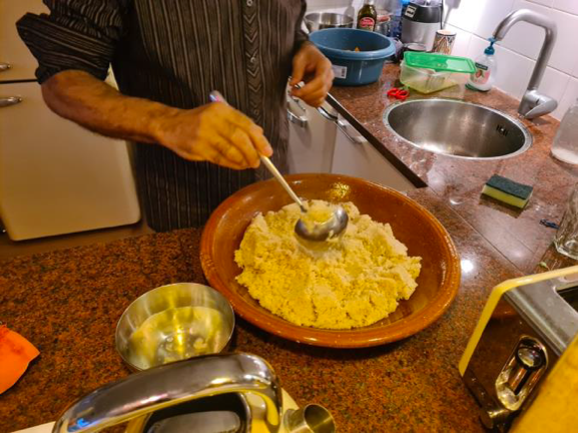
\includegraphics[width=\linewidth]{hoofdgerechten/fotos/couscous5.png}
\hspace{1cm}\newline

\vspace*{\fill}\switchcolumn

{\renewcommand{\arraystretch}{2}
    \begin{tabularx}{\linewidth}{YYY} % Y is custom column that is centered
        \rowcolor[RGB]{236, 234, 231}
         Voorbereiding: & Bereiding: & Totale tijd: \\ 
         10 min & 1 tot 2 uur & 2 uur \\
         \hline
    \end{tabularx}
}

\hspace{1cm}\newline

% TODO: crop bottom of picture to be x cm tall
% https://tex.stackexchange.com/questions/57418/crop-an-inserted-image
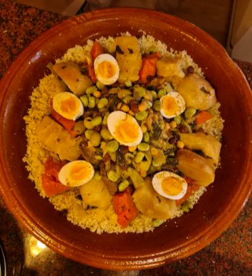
\includegraphics[width=\linewidth]{hoofdgerechten/fotos/couscous1.png}

\hspace{1cm}\newline

\uppercase{\textbf{Bereiden}}
\begin{enumerate}
    \item Snij eerst de uien in grove parten en snij/pers de knoflook fijn (dit gaan straks bij de gemarineerde kip).
    \item Begin nu met het marineren van de kip. Doe de kip in een schaal en doe hierbij de olijfolie en grote theelepels kurkuma, gemalen koriander, komijnpoeder, karwijzaadpoeder, paprikapoeder, gemberpoeder, zwarte peper en een snufje cayennepeper. Voeg ook de fijngesneden knoflook toe. Meng alles door elkaar en leg er vervolgens de ui parten bovenop. Dek af en zet in de koelkast.
    \item Meng alle kruiden in dezelfde hoeveelheden, maar dan kleine theelepels, in een apart klein schaaltje en bewaar dit voor later.
    \item Snij dan de groenten in grove stukken en bewaar voor later.
    \item Doe de couscous in een couscousschaal en giet er wat koud water over waardoor het net onder staat. Laat dit ongeveer 15 minuten intrekken. Maak vervolgens de couscous los.
    \item Breng water aan de kook in de onderste helft van de pan. Vul de bovenste helft van de pan met de couscous uit de couscousschaal en maak er wat gaten in tot de bodem met de achterkant van een pollepel. Als het water kookt zet je de couscous op de onderste helft van de pan en laat je deze 20 tot 30 minuten stomen.
    \item Haal na het stomen de couscous uit de pan en kiep deze om in de couscousschaal. Schep om met een lepel. Pak een kopje gekookt/heet water (kan ook uit de pan) en voeg hier een theelepeltje zout aan toe. Voeg dit vervolgens gelijkmatig toe aan de couscous in de couscousschaal en schep om. Voeg ook wat olijfolie toe en schep weer om. Laat afkoelen.
    \item Gooi ondertussen de onderste helft van de pan leeg. Leg hier vervolgens de gemarineerde kip met uien in en zet het vuur aan. Bak de kip 1 minuut. Voeg vervolgens water toe tot de kip bijna onder staat. Leg hier alvast de knolselderij en de pompoen bovenop en voeg wat meer water toe. Breng aan de kook.
    \item Doe de couscous uit de couscousschaal terug in de bovenste helft van de pan. Laat deze vervolgens weer 20 tot 30 minuten stomen boven de kip en de groenten.
    \item Haal de couscous uit de pan en kiep om in de couscousschaal. Schep om en laat afkoelen. Voeg eventueel wat olijfolie toe en maak los met je handen zodat zoveel mogelijk klontjes weg zijn.
    \item Voeg ondertussen het aparte schaaltje kruiden toe aan de kip en groenten in de pan. Kruimel hier ook de groentebouillonblokjes boven. Leg de stukken courgette en wortel erbij.
    \item Doe na 10 tot 15 minuten de couscous weer in de bovenste helft van de pan en laat deze weer 20 tot 30 minuten stomen boven de kip en de groenten.
    \item Ondertussen kun je beginnen met het koken van de eieren in een aparte pan of eierkoker. Zorg ervoor dat de eieren medium tot hard gekookt zijn.
    \item Haal de couscous uit de pan en kiep in de couscousschaal. Maak weer los met een lepel en je handen. Zorg ervoor dat de couscous gelijk over de schaal verdeeld is en maak de randen wat hoger met een kuiltje in het midden.
    \item Voeg een handje rozijnen, kikkererwten en tuinbonen toe aan de groenten en verwarm even mee.
    \item Nu kan de couscous opgebouwd worden. Begin met een stapeltje maken van de kip in het midden van de kuil in de schaal. Daaromheen leg je de groenten zodat de kip niet meer te zien is. Gooi hier overheen wat van de saus met kikkererwten, ui, tuinbonen en rozijnen. Je kunt ook wat saus over de couscous doen.
    \item Snij de eieren in de lente doormidden en verdeel over de schaal.
    \item Serveer de saus los in een bakje bij de couscous.
\end{enumerate}

\end{paracol}
